\documentclass[preprint]{sigplanconf}

%% I am getting an error about too many math packages used!!!
%% I commented the ones we don't seem to be using.

\usepackage{graphicx}
%%\usepackage{longtable}
\usepackage{comment}
\usepackage{amsmath}
%%\usepackage{mdwlist}
%%\usepackage{txfonts}
\usepackage{xspace}
%%\usepackage{amstext}
\usepackage{amssymb}
\usepackage{stmaryrd}
\usepackage{proof}
\usepackage{multicol}
\usepackage[nodayofweek]{datetime}
\usepackage{etex}
\usepackage[all, cmtip]{xy}
\usepackage{xcolor}
\usepackage{listings}
\usepackage{multicol}
\newcommand\hmmax{0} % default 3
\newcommand\bmmax{0} % default 4
\usepackage{bm}
\usepackage{cmll}

%% \newtheorem{theorem}{Theorem}[section]
%% \newtheorem{lemma}[theorem]{Lemma}
%% \newtheorem{proposition}[theorem]{Proposition}
%% \newtheorem{corollary}[theorem]{Corollary}

\newcommand{\xcomment}[2]{\textbf{#1:~\textsl{#2}}}
\newcommand{\amr}[1]{\xcomment{Amr}{#1}}
\newcommand{\roshan}[1]{\xcomment{Roshan}{#1}}

\newcommand{\ie}{\textit{i.e.}\xspace}
\newcommand{\eg}{\textit{e.g.}\xspace}

\newcommand{\lcal}{\ensuremath{\lambda}-calculus}
\newcommand{\G}{\ensuremath{\mathcal{G}}\xspace}

\newcommand{\code}[1]{\lstinline[basicstyle=\small]{#1}\xspace}
\newcommand{\name}[1]{\code{#1}}

\def\newblock{}

\newenvironment{floatrule}
    {\hrule width \hsize height .33pt \vspace{.5pc}}
    {\par\addvspace{.5pc}}

\newtheorem{theorem}{Theorem}[section]
\newtheorem{lemma}[theorem]{Lemma}
\newtheorem{definition}[theorem]{Definition}
\newtheorem{proposition}[theorem]{Proposition}
\newenvironment{proof}[1][Proof.]{\begin{trivlist}\item[\hskip \labelsep {\bfseries #1}]}{\end{trivlist}}

\newcommand{\arrow}[1]{\mathtt{#1}}

%subcode-inline{bnf-inline} name langRev
%! swap+ = \mathit{swap}^+
%! swap* = \mathit{swap}^*
%! dagger =  ^{\dagger}
%! assocl+ = \mathit{assocl}^+
%! assocr+ = \mathit{assocr}^+
%! assocl* = \mathit{assocl}^*
%! assocr* = \mathit{assocr}^*
%! identr* = \mathit{uniti}
%! identl* = \mathit{unite}
%! dist = \mathit{distrib}
%! factor = \mathit{factor}
%! eta = \eta
%! eps = \epsilon
%! eta+ = \eta^+
%! eps+ = \epsilon^+
%! eta* = \eta^{\times}
%! eps* = \epsilon^{\times}
%! trace+ = trace^+
%! trace* = trace^{\times}
%! ^^^ = ^{-1}
%! (o) = \fatsemi
%! (;) = \fatsemi
%! (*) = \times
%! (+) = +
%! LeftP = L^+
%! RightP = R^+
%! LeftT = L^{\times}
%! RightT = R^{\times}

%subcode-inline{bnf-inline} regex \{\{(((\}[^\}])|[^\}])*)\}\} name main include langRev
%! Gx = \Gamma^{\times}
%! G = \Gamma
%! [] = \Box
%! |-->* = \mapsto^{*}
%! |-->> = \mapsto_{\ggg}
%! |--> = \mapsto
%! |- = \vdash
%! <><> = \approx
%! ==> = \Longrightarrow
%! <== = \Longleftarrow
%! <=> = \Longleftrightarrow
%! <-> = \leftrightarrow
%! ~> = \leadsto
%! -o = \multimap
%! ::= = &::=&
%! /= = \neq
%! @@ = \mu
%! forall = \forall
%! exists = \exists
%! empty = \epsilon
%! langRev = \Pi
%! langRevT = \Pi^{o}
%! langRevEE = \Pi^{\eta\epsilon}
%! theseus = Theseus
%! sqrt(x) = \sqrt{#x}
%! surd(p,x) = \sqrt[#p]{#x}
%! inv(x) = \frac{1}{#x}
%! frac(x,y) = \frac{#x}{#y}
%! * = \times

%%%%%%%%%%%%%%%%%%%%%%%%%%%%%%%%%%%%%%%%%%%%%%%%%%%%%%%%%%%%%%%%%%%%%%%%%%%%%%%%
\begin{document}

\conferenceinfo{ICFP'12}{}
\CopyrightYear{}
\copyrightdata{}
\titlebanner{}
\preprintfooter{}

\title{The Two Dualities of Computation: Negative and Fractional Types}
\authorinfo{Roshan P. James}
           {Indiana University}
           {rpjames@indiana.edu}
\authorinfo{Amr Sabry}
           {Indiana University}
           {sabry@indiana.edu}
\maketitle

\begin{abstract}
  Every functional programmer knows about sum and product types, {{a+b}} and
  {{a*b}} respectively. Negative and fractional types, $a-b$ and $a/b$
  respectively, are much less known and their computational interpretation is
  unfamiliar and often complicated. We show that in a programming model in
  which information is preserved (such as the model introduced in our recent
  paper on \emph{Information Effects}), these types have particularly natural
  computational interpretations. Intuitively, values of negative types are
  values that flow ``backwards'' to satisfy demands and values of fractional
  types are values that impose constraints on their context.  The combination
  of these negative and fractional types enables greater flexibility in
  programming by breaking global invariants into local ones that can be
  autonomously satisfied by a subcomputation. Furthermore, these types and
  their properties suggest that the previously observed duality of
  computation conflated two orthogonal notions: an additive duality that
  corresponds to backtracking and a multiplicative duality that corresponds
  to unification.
\end{abstract}

\category{D.3.1}{Formal Definitions and Theory}{}
\category{F.3.2}{Semantics of Programming Languages}{}
\category{F.3.3}{Studies of Program Constructs}{Type structure}

\terms
Languages, Theory

\keywords continuations, information flow, linear logic, logic programming,
quantum computing, reversible logic, symmetric monoidal categories, compact
closed categories.

%%%%%%%%%%%%%%%%%%%%%%%%%%%%%%%%%%%%%%%%%%%%%%%%%%%%%%%%%%%%%%%%%%%%%%%%%%%%%%%%
\section{Introduction}

In a recent paper~\cite{infeffects}, we argued that, because they include
irreversible physical primitives, conventional abstract models of computation
have inadvertently included some \emph{implicit} computational effects which
we called \emph{information effects}. We then developed a pure reversible
model of computation that is obtained from the type isomorphisms and
categorical structures that underlie models of linear logic and quantum
computing and that treats information as a linear resource that can neither
be erased nor duplicated. In this paper, we show that our pure reversible
model unveils deeper and more elegant symmetries of computation than have
previously been reported. In particular, we expose two notions of duality of
computation: an additive duality and a multiplicative duality that give rise
to negative types and fractional types respectively. Although these types
have previously appeared in the literature (see Sec.~\ref{sec:related}), they
have typically appeared in the context of conventional languages with
information effects, which obscured their appeal and murked their properties.

To get a feeling for the main idea, consider the following algebraic
manipulation relating a natural number $a$ to itself:
\[\begin{array}{rclll}
&& a & \mbox{initial~$a$} & (0) \\
&=& a + 0 & \mbox{$0$~is~identity~for~$+$} & (1) \\
&=& a + (-a + a) & \mbox{$-a$~is~the~additive~inverse~of~$a$} & (2) \\
&=& (a + (-a)) + a & \mbox{$+$~is~associative} & (3) \\
&=& 0 + a & \mbox{$-a$~is~the~additive~inverse~of~$a$} & (4) \\
&=& a & \mbox{$0$~is~identity~for~$+$} & (5)
\end{array}\]
Although seemingly pointless, this algebraic proof corresponds, in our model,
to an isomorphism of type {{a <-> a}} with a non-trivial and interesting
computational interpretation. Consider the starting value of type $a$ as
being supplied by a producer of values and the final value of type $a$ as
being demanded by a consumer. For the purposes of the example, think of the
producer as someone having \$20.00 and the consumer as someone demanding
\$20.00. It is certainly possible to directly connect the producer and
consumer using the algebraic identity $a=a$: such a connection would be
computationally modeled by the identity function as expected. However, the
algebraic proof above implements this connection in a much more interesting
way. As the semantics of Sec.~\ref{sec:rat} formalizes, the flow of 
computation is as follows:
\begin{itemize}
\item We start at line (0) with \$20.00; 
\item We proceed to line (1) with the same \$20.00 but tagged as being in the
  left summand of the type $a+0$; we indicate this value as {{left 20}}
\item We continue to line (2) with the same value {{left 20}};
\item At line (3), the tag on the \$20.00 changes to indicate that it is
  in the left-left summand, i.e., the value is now {{left (left 20)}};
\item At line (4), we find ourselves needing to produce a value of type 0
  which is impossible; this signals the beginning of a reverse execution
  which sends us back to line (3) with a value {{left (right 20)}};
\item Execution continues in reverse to line (2) with the value 
  {{right (left 20)}};
\item At line (1) we find ourselves again facing an empty type so we reverse
  execution again; we go to line (2) with a value {{right (right 20)}};
\item We proceed to line (3) and (4) with the value {{right 20}};
\item We finally reach line 5 with the value {{20}}.
\end{itemize}
The beauty of the above computation is that it can be realized with a
completely different concurrent schedule as follows. \emph{Simultaneously}
the execution begins at line (0) with the value {{20}}, at line (2) with the
value {{right (right 20)}} flowing forward and the value {{right (left 20)}}
flowing backwards, and at line (3) with the value {{left (left 20)}} flowing
forward and the value {{left (right 20)}} flowing backward. We now have three
independent subcomputations proceeding in parallel: the positive value
created at line (2) which can flow to the consumer; the negative value
created at line (3) which can pay for the debt created at line (2); and the
initial value from line (0) which can flow to the required forward-flowing
value needed at line (3). At some intuitive level, one might understand the
situation as modeling a credit card payment in which money is created at line
(2) for the consumer together with a corresponding debt. The producer's bank
pays for the debt at line (3) and waits for the actual money to arrive from
the producer.

There are at least two fundamental points about this example that must be
emphasized:
\begin{itemize}
\item As the example illustrates, negative types corresponds to ``debts.''
  It would clearly be disastrous if debts could be deleted or
  duplicated. This simple observation explains why negative types are much
  simpler and much more appealing in a framework where information is
  guaranteed to be preserved. In previous work that used negative types (see
  Sec.~\ref{sec:related}), complicated mechanisms are typically needed to
  constrain the propagation and use of negative values because the
  surrounding computational framework is, generally speaking, careless in its
  treatment of information.
\item The appeal of negative types can already be gleaned from the credit
  card analogy. The main reason credit card transactions are convenient is
  because they disentangle the propagation of the resources (money) from the
  propagation of the services. Not every transaction needs both the resources
  and services to be brought together: it is sufficient to have a promise
  that the demand for resources will be somehow satisfied, as long as the
  infrastructure can be trusted with such promises. Computationally, this
  means that negative types allow us to break the dependency between
  producers and consumers and let each compute independently.
\end{itemize}

Instead of also discussing fractional types and related work in this
introduction, we briefly summarize our main technical contributions and move
on to the heart of the paper where these topics can be explained in their
proper context. Our main contributions are:
\begin{itemize}
\item We extend {{langRev}} our reversible programming language of type
  isomorphisms~\cite{rc2011,infeffects} (see Sec.~\ref{sec:pi}) with a notion
  of negative types, that satisfies the isomorphism $a + (-a) = 0$. The
  semantics of this extension is expressed by having a ``dual'' evaluator
  that reverses the flow of execution for negative
  values. (Sec.~\ref{sec:neg})
\item We independently extend {{langRev}} with a notion of fractional types,
  that satisfies the isomorphism $a * (1/a) = 1$. The semantics of this
  extension is expressed by introducing logical variables and a unification
  mechanism to model and resolve the constraints introduced by the fractional
  types. (Sec.~\ref{sec:frac})
\item We combine the above two extensions into one extension that includes
  both negative and fractional types. The resulting language allows any
  rational number to be used as a type. The types satisfy the same familiar
  and intuitive isomorphisms that are satisfied in the mathematical field of
  rational numbers. (Sec.~\ref{sec:rat})
\item We develop programming intuition and argue that negative and fractional
  types ought to be part of the vocabulary of every
  programmer. (Sec.~\ref{sec:prog})
\item We relate our notions of negative and fractional types to previous work
  on continuations. Briefly, we argue that conventional continuations
  conflate negative and fractional components. This observation allows us to
  relate two apparently unrelated lines of work: the first pioneered by
  Filinski~\cite{Filinski:1989:DCI:648332.755574} relating continuations to
  negative types and the second~\cite{Bernardi:2010:CSL:1749618.1749689}
  relating continuations to the fractional types of the Lambek-Grishin
  calculus. (Sec.~\ref{sec:related})
\end{itemize}

%%%%%%%%%%%%%%%%%%%%%%%%%%%%%%%%%%%%%%%%%%%%%%%%%%%%%%%%%%%%%%%%%%%%%%%%%%%%%%%%
\section{The Core Reversible Language: {{langRev}} }
\label{sec:pi}

We review our reversible language {{langRev}}: the presentation in this
section differs from the one in our previous paper~\cite{infeffects} in two
aspects. First, we add the empty type $0$ which is necessary to express the
additive duality. Second, instead of explaining evaluation using a natural
semantics, we give a small-step operational semantics that is more
appropriate for the connections with continuations explored in this paper.

%%%%%%%%%%%%%%%%%%%%
\subsection{Syntax} 

The set of types includes the empty type {{0}}, the unit type {{1}}, sum
types {{b1+b2}}, and products types {{b1*b2}}. The set of values {{v}}
includes {{()}} which is the only value of type {{1}}, {{left v}} and {{right v}} 
which inject {{v}} into a sum type, and {{(v1,v2)}} which builds a
value of product type. There are no values of type {{0}}:
%subcode{bnf} include main
% value types, b ::= 0 | 1 | b + b | b * b 
% values, v ::= () | left v | right v | (v, v)

The combinators of {{langRev}} are witnesses to the following type
isomorphisms: 
%subcode{bnf} include main
%! columnStyle = r@{\hspace{-0.5pt}}c@{\hspace{-0.5pt}}l
%zeroe :&  0 + b <-> b &: zeroi
%swap+ :&  b1 + b2 <-> b2 + b1 &: swap+
%assocl+ :&  b1 + (b2 + b3) <-> (b1 + b2) + b3 &: assocr+
%identl* :&  1 * b <-> b &: identr*
%swap* :&  b1 * b2 <-> b2 * b1 &: swap*
%assocl* :&  b1 * (b2 * b3) <-> (b1 * b2) * b3 &: assocr*
%dist0 :& 0 * b <-> 0 &: factor0
%dist :&~ (b1 + b2) * b3 <-> (b1 * b3) + (b2 * b3)~ &: factor
Each line of the above table introduces one or two combinators that witness
the isomorphism in the middle. Collectively the isomorphisms state that the
structure {{(b,+,0,*,1)}} is a \emph{commutative semiring}, i.e., that each
of {{(b,+,0)}} and {{(b,*,1)}} is a commutative monoid and that
multiplication distributes over addition. The isomorphisms are extended to
form a congruence relation by adding the following constructors that witness
the equivalence and compatible closure:
%subcode{proof} include main
%@  ~
%@@ id : b <-> b 
%
%@ c : b1 <-> b2
%@@ sym c : b2 <-> b1
%
%@ c1 : b1 <-> b2
%@ c2 : b2 <-> b3
%@@ c1(;)c2 : b1 <-> b3
%---
%@ c1 : b1 <-> b3
%@ c2 : b2 <-> b4
%@@ c1 (+) c2 : b1 + b2 <-> b3 + b4
%
%@ c1 : b1 <-> b3
%@ c2 : b2 <-> b4
%@@ c1 (*) c2 : b1 * b2 <-> b3 * b4

To summarize, the syntax of {{langRev}} is given as follows. 

\begin{definition}{(Syntax of {{langRev}})}
\label{def:langRev}
We collect our types, values, and combinators, to get the full language
definition.
%subcode{bnf} include main
% value types, b ::= 0 | 1 | b+b | b*b 
% values, v ::= () | left v | right v | (v,v) 
%
% comb.~types, t ::= b <-> b
% iso ::= zeroe | zeroi 
%     &|& swap+ | assocl+ | assocr+ 
%     &|& identl* | identr* 
%     &|& swap* | assocl* | assocr* 
%     &|& dist0 | factor0 | dist | factor 
% comb., c ::= iso | id | sym c | c (;) c | c (+) c | c (*) c 
\end{definition}

%%%%%%%%%%%%%%%%%%%%%%%%%%%%%%%%%%%%%%%%%%%%%%%%%%%%%%%%%%%%%%%%%%%%%%%%%%%%%%
\subsection{Graphical Language}

The syntactic notation described above is often obscure. Following the
tradition established for monoidal
categories~\cite{springerlink:10.1007/978-3-642-12821-94}, we present a
graphical language that conveys the intuitive semantics of the language
(which is formalized in the next section). The general idea of the graphical
notation is that combinators are modeled by ``wiring diagrams'' or
``circuits''; values are modeled as ``particles'' that may appear on the
wires; and evaluation is modeled by the flow of particles along the wires. We
now proceed to give the graphical notation for each combinator:

\begin{itemize}
\item The simplest sort of diagram is the {{id : b <-> b}} combinator which
  is simply represented as a wire labeled by its type {{b}}. In more complex
  diagrams, if the type of a wire is obvious from the context, it may be
  omitted.
\begin{center}
\scalebox{0.95}{
%%subcode-line{pdfimage}[diagrams/thesis/b-wire.pdf]

\includegraphics{diagrams/thesis/b-wire.pdf}
}
\end{center}

\item The product type {{b1*b2}} may be represented both as one wire labeled
  {{b1*b2}} or by two parallel wires labeled {{b1}} and {{b2}}. Both
  representations maybe used interchangeably.
\begin{multicols}{2}
\begin{center}
\scalebox{0.95}{
%%subcode-line{pdfimage}[diagrams/thesis/pair-one-wire.pdf]

\includegraphics{diagrams/thesis/product-one-wire.pdf}
}
\end{center}
\begin{center}
\scalebox{0.95}{
%%%subcode-line{pdfimage}[diagrams/thesis/pair-of-wires.pdf]
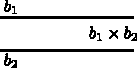
\includegraphics{diagrams/thesis/product-two-wires.pdf}
}
\end{center}
\end{multicols}

\item Sum types may similarly be represented by one wire or using using
  parallel wires with a {{+}} operator between them.
\begin{multicols}{2}
\begin{center}
\scalebox{0.95}{
%%subcode-line{pdfimage}[diagrams/thesis/sum-one-wire.pdf]

\includegraphics{diagrams/thesis/sum-one-wire.pdf}
}
\end{center}
\begin{center}
\scalebox{0.95}{
%%subcode-line{pdfimage}[diagrams/thesis/sum-of-wires.pdf]
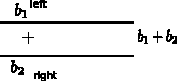
\includegraphics{diagrams/thesis/sum-two-wires.pdf}
}
\end{center}
\end{multicols}

%% \item
%% When representing complex types like {{(b1*b2)+b3}} some visual
%% grouping of the wires may be done to aid readability. The exact type
%% however will always be clarified by the context of the diagram.

%% \begin{center}
%% \scalebox{0.95}{
%% %subcode-line{pdfimage}[diagrams/thesis/complex-type-crop.pdf]
%% }
%% \end{center}

\item Associativity is implicit in the graphical language. Three parallel
  wires represent {{b1*(b2*b3)}} or {{(b1*b2)*b3}}, based on the context.
\begin{center}
\scalebox{0.95}{
%%subcode-line{pdfimage}[diagrams/thesis/associate.pdf]
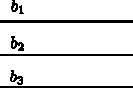
\includegraphics{diagrams/thesis/assoc.pdf}
}
\end{center}

\item Commutativity is represented by crisscrossing wires.
\begin{multicols}{2}
\begin{center}
\scalebox{0.95}{
%%subcode-line{pdfimage}[diagrams/thesis/swap-pair.pdf]
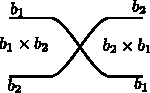
\includegraphics{diagrams/thesis/swap_times.pdf}
}
\end{center}
\begin{center}
\scalebox{0.95}{
%%subcode-line{pdfimage}[diagrams/thesis/swap-sum.pdf]
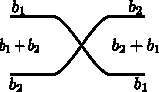
\includegraphics{diagrams/thesis/swap_plus.pdf}
}
\end{center}
\end{multicols}

\item Identity morphisms and their duals ({{uniti, unite, zeroi}} and
  {{zeroe}}) are represented as follows:
\begin{multicols}{2}
\begin{center}
\scalebox{0.95}{
%%subcode-line{pdfimage}[diagrams/thesis/identr1.pdf]
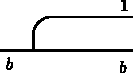
\includegraphics{diagrams/thesis/uniti.pdf}
}
\end{center}
\begin{center}
\scalebox{0.95}{
%%subcode-line{pdfimage}[diagrams/thesis/identl1.pdf]
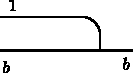
\includegraphics{diagrams/thesis/unite.pdf}
}
\end{center}  
\end{multicols}
\begin{multicols}{2}
\begin{center}
\scalebox{0.95}{
%%subcode-line{pdfimage}[diagrams/thesis/identr0.pdf]
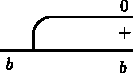
\includegraphics{diagrams/thesis/zeroi.pdf}
}
\end{center}
\columnbreak
\begin{center}
\scalebox{0.95}{
%%subcode-line{pdfimage}[diagrams/thesis/identl0.pdf]
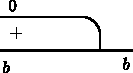
\includegraphics{diagrams/thesis/zeroe.pdf}
}
\end{center}
\end{multicols}
Since the monoidal units can be freely introduced and eliminated, in
many diagrams they are omitted and dealt with explicitly when they
are of special interest.

\item Finally, distributivity and factoring are represented using the dual
  boxes shown below:
\begin{multicols}{2}
\begin{center}
\scalebox{0.95}{
%%subcode-line{pdfimage}[diagrams/thesis/distrib-crop.pdf]
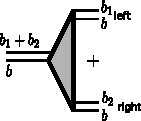
\includegraphics{diagrams/thesis/dist.pdf}
}
\end{center}
\begin{center}
\scalebox{0.95}{
%%subcode-line{pdfimage}[diagrams/thesis/factor-crop.pdf]
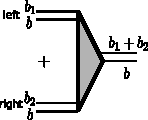
\includegraphics{diagrams/thesis/factor.pdf}
}
\end{center}
\end{multicols}

\end{itemize}

\noindent 
\textit{Example.} As an example, the following combinator is represented by
the given diagram:

{{c : b * (1+1) <-> b + b}}

{{c = swap* (;) dist (;) (identl* (+) identl*)}}

\begin{center}
\scalebox{0.95}{
%%subcode-line{pdfimage}[diagrams/thesis/example1-crop.pdf]
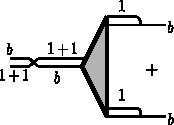
\includegraphics{diagrams/thesis/example1.pdf}
}
\end{center}

%%%%%%%%%%%%%%%%%%%%%%%%%%%%%%%%%%%%%%%%%%%%%%%%%%%%%%%%%%%%%%%%%%%%%%%%%%%%
\subsection{Semantics}

The semantics of the primitive combinators is given by the following
single-step reductions. Since there are no values of type {{0}}, the rules
omit some of the impossible cases:
\begin{scriptsize}
%subcode{opsem} include main
%! columnStyle = rlcl
% swap+ & (left v) &|-->& right v
% swap+ & (right v) &|-->& left v 
% assocl+ & (left v1) &|-->& left (left v1)
% assocl+ & (right (left v2)) &|-->& left (right v2)
% assocl+ & (right (right v3)) &|-->& right v3 
% assocr+ & (left (left v1)) &|-->& left v1
% assocr+ & (left (right v2)) &|-->& right (left v2)
% assocr+ & (right v3) &|-->& right (right v3)
% identl* & ((), v) &|-->& v 
% identr* & v &|-->& ((), v) 
% swap* & (v1, v2) &|-->& (v2, v1) 
% assocl* & (v1, (v2, v3)) &|-->& ((v1, v2), v3) 
% assocr* & ((v1, v2), v3) &|-->& (v1, (v2, v3)) 
% dist & (left v1, v3) &|-->& left (v1, v3)
% dist & (right v2, v3) &|-->& right (v2, v3)
% factor & (left (v1, v3)) &|-->& (left v1, v3) 
% factor & (right (v2, v3)) &|-->& (right v2, v3)   
\end{scriptsize}

For the non-primitive combinators, we express the semantics using evaluation
contexts which are used to represent the ``rest of the computation.'' More
precisely, to calculate the result of applying combinator $c$ to value $v$,
we start a small-step abstract machine in the configuration . The
transitions of the machine (see below) are unusual in the sense that they
always maintain full information about {{c}}, although this information may
be split in the first and last component of the machine. The {{v}} component
of the machine is the one that captures the current value as it is flowing in
the combinator {{c}}. When  scattered in the machine will examine {{c}} and make
transitions based on the structure of {{c}}. When the evaluation of {{c}} is
complete, the configuration should be {{[c,v,[]]}} where the {{c}} is
restored.

This is a mess. Perhaps give a small example and explain things based on the
example before giving the full transitions.


%subcode{bnf} include main
% Combinator Contexts, C = [] | Fst C c | Snd c C 
%                  &|& LeftT C c v | RightT c v C 
%                  &|& LeftP C c | RightP c C 
% Machine states = <c, v, C> | {[c, v, C]}
% Start state = <c, v, []> 
% Stop State = {[c, v, []]}


%subcode{opsem} include main
%! columnStyle = rclr
% <iso, v, C> &|-->& {[iso, iso(v), C]}
% <c1(;)c2, v, C> &|-->& <c1, v, Fst C c2>
% {[c1, v, Fst C c2]} &|-->& <c2, v, Snd c1 C>
% {[c2, v, Snd c1 C]} &|-->& {[ c1(;)c2, v, C ]}
% <c1(+)c2, left v, C> &|-->& <c1, v, LeftP C c2>
% {[ c1, v, LeftP C c2 ]} &|-->& {[c1 (+) c2, left v, C ]}
% <c1(+)c2, right v, C> &|-->& <c2, v, RightP c1 C>
% {[ c2, v, RightP c1 C ]} &|-->& {[c1 (+) c2, right v, C ]}
% <c1(*)c2, (v1, v2), C> &|-->& <c1, v1, LeftT C c2 v2>
% {[ c1, v1, LeftT C c2 v2 ]} &|-->& <c2, v2, RightT c1 v1 C>
% {[ c2, v2, RightT c1 v1 C ]} &|-->& {[ c1 (*) c2, (v1, v2), C ]}

\begin{proposition}[Logical Reversibility]
\label{prop:logrev}
{{c v |--> v'}} iff {{c{dagger} v' |--> v}}.
\end{proposition}

\roshan{We really have to rethink this prop in the precense of
  negatives and fractionals. With negatives, the program can actually
  end at the begining of the circuit -- i.e. the program {{c:b1<->b2}}
  can stop with a value of type {{b1}}. With fractionals, there can be
  several values of type {{b2}} produced for a value of type {{b1}}. }

\begin{proposition}[Groupoid]
\label{prop:groupoid}
{{langRev}} is a groupoid. 
\end{proposition}

\begin{proposition}
\label{prop:category}
{{langRev}} is a dagger symmetric monoidal category. 
\end{proposition}

%%%%%%%%%%%%%%%%%%%%%%%%%%%%%%%%%%%%%%%%%%%%%%%%%%%%%%%%%%%%%%%%%%%%%%%%%%%%%%%%
\section{Negative Types}
\label{sec:neg}

Consider the following two ways of purchasing an item that costs \$20.00:
\begin{enumerate}
\item You give the seller a \$20.00 bill.
\item You use a credit card to pay the seller.
\end{enumerate}
In both cases, the seller receives the money immediately but there is a
subtle difference. In the first transaction, the money received by the seller
corresponds to a value that has been produced earlier in the computation. In
the second transaction, the money may or may not exist yet: computationally,
a \emph{debt} is generated to compensate for the money received by the seller
and this debt travels ``backwards'' towards the bank where it is (hopefully)
reconciled.

The example suggests that the ability to consider values flowing backwards
enriches our computational model. This observation goes back to Filinski's
Masters thesis where continuations are identified with these negative values.
We discuss the connections to Filinski's work and others in more detail in
Sec.~\ref{sec:related}. For now, we note that in a conventional programming
language in which values can be copied and deleted at will, extreme care is
needed to keep track of negative values. Indeed, in the example above, if it
were possible to simply delete the variable corresponding to the debt, we
would have produced money out of nothing. 

For this reason, our treatment of negative values in the context of
{{langRev}} is particularly simple. We will have a type $0$ and an
isomorphism {{0 <-> a + (-a)}} that when used in the left-to-right direction
allows us to create a value and a corresponding debt out of nothing. Both the
value and its negative counterpart can flow anywhere in the system. Because
information is preserved, a closed program (which does not have any
``dangling'' negative values) will eventually have to match the negative
value with some corresponding value, effectively using the isomorphism in the
right-to-left direction. In more detail, we can model the credit card
transaction above using the following program (shown diagrammatically):

\begin{center}
  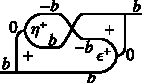
\includegraphics{diagrams/algebra1.pdf}
\end{center}

\roshan{I chose to draw the igure with b instead of a, since b is what
  we use for the types. Should this be a? Also I chose to make the
  swap and 0 wires, explicit.Is this what you intended? }


CLEAN UP the following based on the figure. In contrast, in our setting, one
can start from the empty type $0$, introduce a positive value and its
negative counterpart, and let each of these flow in arbitrary ways. The
entire framework guarantees that neither the value nor its negative
counterpart will be deleted or duplicated and hence that, in any closed
program, the ``debt'' corresponding to the negative value is paid off exactly
once. Computationally we model the first transaction using essentially the
identity function which receives a \$20.00 bill as input from the buyer and
propagates it on its output to the seller. The second transaction is more
complicated. We model it as shown in the circuit below: There are two ways to
understand this circuit that are both quite instructive. Let's first examine
the type structure of each of the combinators that comprise the circuit. The
first combinator on the right outputs \$20.00 to the seller. This \$20.00 is
produced from nothing so to speak by generating an equivalent debt that
travels backwards. COMPLETE BASED ON THE FIGURE. The other way is to follow
the execution. It goes forward in time so to speak, comes back, and then goes
forwards again.

It is critical that the framework in which the negative types are introduced
is a framework in which all information is preserved, with no duplication or
erasure. This guarantees that the generated debts are paid once and exactly
once.

%%%%%%%%%%%%%%%%%%%%%%%%%%%%
\paragraph*{Observability.} 
Execution of program is defined by {{c : b1 <-> b2}} when evaluated on input
{{v1 : b1}} gives us a value {{v2 : b2}} on termination. Execution is well
defined only if {{b1}} and {{b2}} are entirely positive types. This is
similar to the constraint that Zeilberger imposes to explain intuitionistic
polarity and delimited control~\cite{10.1109/LICS.2010.23}.

Consider the program that

(TODO: So this is a really bad explanation. But this section is really
important and we need to explain carefully. Maybe an analogy can be
drawn to Cayley diagrams for groups to point out that the notion of
`i' is entirely artificial, but it is essential to the discourse.)

\begin{center}
  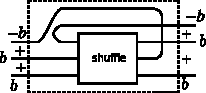
\includegraphics{diagrams/shuffle.pdf}
\end{center}

We define observables to be only positive types. The outputs of
programs that output mixed positive and negative types are not
observable.  Also, programs that input mixed positive and negatives
types are not executable.

%%%%%%%%%%%%%%%%%%%%%%%
\subsection{Additive Duality in {{langRev}} }

Additive duality is added to {{langRev}} by addition of negative types
denoted {{-b}} and the isomorphisms {{eta+}} and {{eps+}}. Hence we
extend the language as follows:

%subcode{bnf} include main
% Value Types, b = ... | -b
% Values, v = ... | -v
%
% Isomorphisms, iso &=& ... | eta+ | eps+

\noindent
with the types judgments

%subcode{opsem} include main
% eta+ &: 0 <-> (-b) + b :& eps+

%subcode{proof} include main
%@ |- v : b
%@@ |- -v : -b

We visually present {{eta+}} and {{eps+}} as `U'-shaped connectors. On
the left below is {{eta+}} showing the map from {{0}} to {{-b+b}} and
dually on the right is {{eps+}} showing the map from {{-b+b}} to
0. Even though the diagrams below show a {{0}} wire for completeness,
later diagrams will always drop them in contexts where we can
implicitly introduce/eliminate then using {{zeroi}}/{{zeroe}}.

\begin{multicols}{2}
\begin{center}
  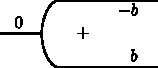
\includegraphics{diagrams/eta.pdf}
\end{center}
  
\begin{center}
  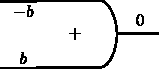
\includegraphics{diagrams/eps.pdf}
\end{center}
\end{multicols}

The usual interpretation of the type {{b1+b2}} is that we either have
an appropriately tagged value of type {{b1}} or an appropriately
tagged value of type {{b2}}. This interpretation is maintained in the
presence of {{eta+}} and {{eps+}} in the following sense: a value of
type {{right v : -b + b}} flowing into an {{eps+}} on the lower wire
switches into a value {{left (-v): -b + b}} that flows backwards on the
upper wire. The inversion of direction is captured by the negative
sign on the value.

\paragraph*{Negative Information Flow.} 
Hence, the intuitive way to read the diagrams is that they reverse the
flow of information -- in normal {{langRev}} circuits information
flows from left-to-right and {{eps+}} operations cause information to
flow from right-to-left.  The interpretation of {{eta+}} is precisely
the opposite: it turns a right-to-left flow of information in a
circuit into a left-to-right flow.

\begin{multicols}{2}
\begin{center}
\scalebox{1.5}{
  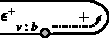
\includegraphics{diagrams/eps_plus1.pdf}
}
\end{center}
  
\begin{center}
\scalebox{1.5}{
  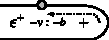
\includegraphics{diagrams/eps_plus2.pdf}
}
\end{center}  
\end{multicols}

\paragraph*{Time Traveling.}
A time traveling intuition is also applicable here: if view the
left-to-right direction of information flow as the canonical forward
direction of information, then the action of {{eps+}} allows values,
aka information particles, to flow backwards in time. Particles that
flow backward in time get to see and interact with the history of
particles that they coexist with i.e. values that they exist
multiplicatively with. Hence the isomorphism {{(-b1)*b2<->-(b1*b2)}}
(whose construction is shown in Section \ref{sec:neg-constructions}).

\paragraph*{Coherence.}
The appropriate coherence condition for Compact Closed Categories,
expressed as the triangle axiom, is satisfied by {{eta+}}/{{eps+}} and
may be visualized as explained by Selinger
\cite{springerlink:10.1007/978-3-642-12821-94} as follows:

\begin{center}
  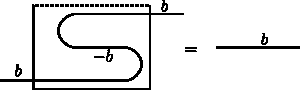
\includegraphics{diagrams/coherence.pdf}
\end{center}

\paragraph*{Non-termination.}
As is well known in category theory, Compact Closed Categories contain
trace operations.  In the context of {{langRev}} this implies that
{{eta+}}/{{eps+}} allow the construction of a {{trace+}} operator
(detailed in Section \ref{sec:monoidal-constructions}) hence
introducing \emph{non-termination} into the language
\cite{infeffects}.

\paragraph*{Zero Information.}
The fact that {{eta+}} (and hence {{eps+}}) introduces no information
can be understood is by viewing {{-b+b}} as a type whose value is
observable only if you `pay' {{b}} amount of information to the {{-b}}
branch. When {{b}} amount of information is supplied {{(-b+b)+b=b}}
amount of information is returned to you. (TODO. more needs to be said
here.)

ADD MATH. 

%%%%%%%%%%%%%%%%%%%%%%%%%%%%%%%%%%%%%%%%%%%%%%%%%%%%%%%%%%%%%%%%%%%%%%%%%%%%%%%%%%%%
\section{Fractional Types}
\label{sec:frac}

The type $a/b$ is prominent in the Lambek-Grishin calculus which is
extensively used in computational linguistics. In the common interpretation,
a value of type $a/b$ is a value of some type $c$ such that when put in a
context of type $b$, the result is a value of type $a$. For example, assuming
contexts are represented as functions, a value of type $\texttt{bool} /
(\texttt{int} \rightarrow \texttt{bool})$ is simply a value of type
$\texttt{int}$. Indeed in this case, putting a value of type $\texttt{int}$
in the context $(\texttt{int} \rightarrow \texttt{bool})$ produces a value of
type $\texttt{bool}$. 

In our case, the situation is simpler. If the goal is to produce a value of
type {{a * b}} and a subcomputation can only produce the {{a}}-part, it would
have type {{(a * b) / b}}. In most settings, this type would be equivalent to
{{a}}. However in our setting, the constraint that this value must eventually
fit in a larger value that supplies the {{b}} is explicitly recorded and must
be resolved. In more detail, we have an isomorphism {{ 1 <-> a * (1/a) }}
which when used in the left-to-right direction allows the creation of a value
and a corresponding constraint on the context.  Both the value and the
constraint can flow in arbitrary ways during the computation but eventually
in a closed program with no ``dangling'' constraints, the isomorphism should
be used in the right-to-left direction to resolve the constraints.  To
understand the computational interpretation, consider the following example.

The goal is to produce a value of type $(\texttt{bool} \times
\texttt{int})$. One part of the program, $e_1$, knows how to produce the
value of type $\texttt{int}$ (say {{3}}) and another part, $e_2$, knows how
to produce the value of type $\texttt{bool}$ (say true). Computationally, we
model this as follows. The first subcomputation $e_1$ produces {{((),3)}} and
uses the isomorphism to convert {{()}} to $(\alpha,1/\alpha)$ where $\alpha$
is a yet-unknown boolean value. Reshuffling the components, $e_1$ produces
$((\alpha,3), 1/\alpha)$. Similarly, $e_2$ can independently produce
$((true,\beta),1/\beta)$ where $\beta$ is a yet-unknown integer value.  When
the two values meet, we can group the components as follows:
\[
(\alpha,\beta)  \qquad (3,1/\beta)  \qquad (true,1/\alpha)
\]
Using the isomorphism in the right-to-left direction on the last two pairs,
forces $\alpha$ to be resolved to true and forces $\beta$ to be resolved to
{{3}}. Both of these pairs then become {{()}} and be absorbed. We are left
with the pair $(true,3)$ as desired.

To summarize, one can think of a value of type $a/b$ as a value that imposes
a constraint on its context of use: it is a value that requires its context
to be of type $b$ and only if that condition is satisfied, can the value be
considered as a value of type $a$. In the simplest case, the type $1/b$ just
constraints the context to be of type $b$. By allowing the fractional types
to be first-class, we can separate the generation of constraints from their
use. Both the value and the constraint can flow in arbitrary ways during the
computation but eventually in a closed program with no ``dangling''
constraints, the isomorphism should be used in the right-to-left direction to
resolve the constraints.

NEED to work out the example in detail (or perhaps another example that's
better. 

Again it is critical that the framework in which the fractional types are
introduced is a framework in which all information is preserved, with no
duplication or erasure. This guarantees that the generated constraints are
satisfied once and exactly once. 

%%%%%%%%%%%%%%%%%%%%%
\subsection{Multiplicative Duality in {{langRev}} }

Multiplicative duality is added to {{langRev}} by adding types
{{b^^^}}, values {{v^^^}} and isomorphisms {{eta*}} and {{eps*}}.
Note that we will freely write {{b^^^}} as {{1/b}} and {{a*b^^^}} as
{{a/b}}.

%subcode{bnf} include main
% Value Types, b = ... | inv(b)
% Values, v = ... | inv(v)
%
% Isomorphisms, iso &=& ... | eta* | eps*

\noindent
These have the type judgments

%subcode{opsem} include main
% eta* &: 1 <-> inv(b) * b :& eps*

%subcode{proof} include main
%@ |- v : b
%@@ |- inv(v) : inv(b)

As with additive duals, we represent {{eta*}} and {{eps*}} using
`U'-shaped connectors. In the general case the wires for {{1}} will be
dropped as it can freely introduced or eliminated using {{uniti}} and
{{unite}}. 

\begin{multicols}{2}
\begin{center}
  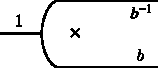
\includegraphics{diagrams/eta_times.pdf}
\end{center}
  
\begin{center}
  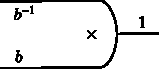
\includegraphics{diagrams/eps_times.pdf}
\end{center}
\end{multicols}

The usual interpretation of {{b1*b2}} we have both a value of type
{{b1}} and a value of type {{b2}}. This interpretation is maintained
in the presence of fractionals. Hence an {{eta* : 1 <-> inv(b) * b}} is
to be viewed as a fission point for a value of type {{b}} and its
multiplicative inverse {{inv(b)}}. This naturally raises the question --
which value of type {{b}} is produced? The isomorphism {{eta*}} does
not produce any specific value of type {{b}}, instead it produces a
place holder for a value such that the value of type {{inv(b)}} is
always the dual of the chosen one. 

\begin{multicols}{2}
\begin{center}
\scalebox{1.5}{
  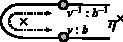
\includegraphics{diagrams/eta_times1.pdf}
}
\end{center}

\begin{center}
\scalebox{1.5}{
  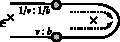
\includegraphics{diagrams/eps_times1.pdf}
}
\end{center}  
\end{multicols}

\paragraph*{Unification.}
A computational interpretation of this is that {{langRevEE}} acts like
a logic programming system and {{eta*}} acts as the site of creation
of a new typed logic variable of type {{b}} and its corresponding dual
of type {{inv(b)}}. These two values are free to move independently
through a circuit, but any operations on value affect what operations
are possible on the other since they are both related by an underlying
logic variable. Dually, {{eps*}} acts as a unification site for values
flowing along both branches. If the values are not exactly duals, then
the system fails to unify and hence the program is stuck. If the
values are exactly duals, then unification succeeds and {{eta*}}
returns {{1}}.

\paragraph*{Entanglement and Anti-Particles.}
A dual view of the operation of {{eta*}} and {{eps*}} is inspired by
quantum mechanics. The {{eta*}} is a site of fission that creates an
information particle and its anti-particle. Both flow in the same
direction in time. The produce particles are entangles in that actions
on one (such as transformation by application of an isomorphism)
affects the other. Further the fission site does not create a particle
in any specific state, but in a superposition of all possible states
as dictated by its type. In each possible world that the particle
exists, it takes on a specific value inhibiting its type and
correspondingly its entangled anti-particle takes the dual of the
specific value.

This also leads to the exciting point of view that entangled
particle/anti-particle pairs act as functions in a physical
first-class sense. We can ask the function to be applied to a value by
unifying the anti-particle with a particle in a well-known state and
examining is pair. We shall use this point of view in the development
our SAT solver (see Sec. \ref{sec:sat-solver}).

\paragraph*{Coherence.} 
As before, the requisite coherence condition on Compact Closed
Categories is applicable and is expressed below in terms of
{{eta*}}/{{eps*}} and the multiplicative monoid.

\begin{center}
  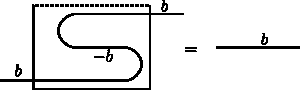
\includegraphics{diagrams/coherence.pdf}
\end{center}

\paragraph*{Annihilation.}
As with {{(+, 0)}} we can construct a {{trace*}} operation. Unlike the
additive {{trace+}}, {{trace*}} gives us the ability to find the
fixpoint of the constraint (expressed with combinators) that is
traced. If the constraint has not satisfying values, there is not
fixpoint possible -- we use the term `annihilation' to describe the
corresponding undefined state of the program. Annihilation and a
non-termination both describe undefined program execution -- while
non-termination characterizes an iteration that fails to terminate,
annihilation characterizes a constraint that has no fixpoint. 

\paragraph*{Zero Information.}
As with {{eta+}}, we argue that {{eta*}} constructs no new
information, instead it gives us the ability to explore as many worlds
as permitted by the type {{b}}. So situate ourselves in any specific
world, we have to supply additional information in the form of
unifying the particle or anti-particle with a particle representing
known information. Hence only by supplying information to a an
entangled pair can we read information from it -- and always exactly
as much information as we supplied.

ADD MATH. 

%%%%%%%%%%%%%%%%%%%%%%%%%%%%%%%%%%%%%%%%%%%%%%%%%%%%%%%%%%%%%%%%%%%%%%%%%%%%%%%%
\section{Rational Types}
\label{sec:rat}

In this section we develop the semantics for {{langRev}} extended with
negative and fractional types, {{langRevEE}}.  We start with the
semantics for {{langRev}} defined in Sec \ref{sec:pi}, which we will
systematically rewrite until we have the desired {{langRevEE}}
sematics. Broadly this construction takes two steps 

\begin{enumerate}
\item We rewrite the semantics in Sec \ref{sec:pi} using unification
  of the values instead of direct pattern matching. This gives us the
  neccessary infrastructure for fractional types, as we will see. 

\item We write a reverse interpreter by reversing the direction of the
  `{{|-->}}' reductions. This gives us the neccessary infrastructure for
  negative types.
\end{enumerate}


%%%%%%%%%%%%%%%%%%%%%%%%%%%%%%%%%%%%%%%%%%%%%%%%%%%%%%%%%%%%%%%%%%%%%%%%%%%%%%%%
\subsection{Unification and Logic Programming}



%%%%%%%%%%%%%%%%%%%%%%%%%%%%%%%%%%%%%%%%%%%%%%%%%%%%%%%%%%%%%%%%%%%%%%%%%%%%%%%%
\subsection{Extending {{langRev}} Semantics}


\paragraph{Primitive Isomorphsims.}
Previously the reductions of the primitive isomorphisms were specified
in the following form.

{{ iso v_{input pattern} |--> v_{output pattern} }}

\noindent
In the precense of unification, we rewrite them to accept the incoming
substitution and extend it with the appropriate unification.

{{ iso s v' |--> (v_{output pattern}, s[v' <><> v_{input pattern}]) }}


\paragraph{Extending the evaulator with unification.} 
We have rewriten the semantics of Sec. \ref{sec:pi} with
unification. The behaviour of the intepreter has not changed.

%subcode{opsem} include main
%! columnStyle = rclr
%! fwd = \triangleright
% <iso, v, C, s>_{fwd} &|-->& {[iso, v', C, s']}_{fwd}
% & & where iso s v |--> (v', s')
% <c1(;)c2, v, C, s>_{fwd} &|-->& <c1, v, Fst C c2, s>_{fwd}
% {[c1, v, Fst C c2, s]}_{fwd} &|-->& <c2, v, Snd c1 C, s>_{fwd}
% {[c2, v, Snd c1 C, s]}_{fwd} &|-->& {[ c1(;)c2, v, C,s ]}_{fwd}
% <c1(+)c2, v', C, s>_{fwd} &|-->& <c1, v, LeftP C c2, s[v' <><> left v]>_{fwd}
% {[ c1, v, LeftP C c2, s ]}_{fwd} &|-->& {[c1 (+) c2, left v, C,s ]}_{fwd}
% <c1(+)c2, v', C, s>_{fwd} &|-->& <c2, v, RightP c1 C, s[v' <><> right v]>_{fwd}
% {[ c2, v, RightP c1 C,s ]}_{fwd} &|-->& {[c1 (+) c2, right v, C,s ]}_{fwd}
% <c1(*)c2, v', C, s>_{fwd} &|-->& <c1, v1, LeftT C c2 v2, s'>_{fwd}
% & & where s' = s[v <><> (v1, v2)]
% {[ c1, v1, LeftT C c2 v2,s ]}_{fwd} &|-->& <c2, v2, RightT c1 v1 C, s>_{fwd}
% {[ c2, v2, RightT c1 v1 C,s ]}_{fwd} &|-->& {[ c1 (*) c2, (v1, v2), C,s ]}_{fwd}

\paragraph{Backward evaluator.}
Here we have written a ``backward'' evaluator in the same style --
i.e. evaluation {{c v}} in this evaluator is equivalent to evaluating
{{C^{dagger} v}} in the forward evaluator.

%subcode{opsem} include main
%! columnStyle = rclr
%! bck = \triangleleft
% {[iso, v, C, s]}_{bck} &|-->& <iso, v', C, s'>_{bck}
% & & where iso^{dagger} s v |--> (v', s')
% <c1, v, Fst C c2, s>_{bck} &|-->& <c1(;)c2, v, C, s>_{bck}
% <c2, v, Snd c1 C, s>_{bck} &|-->& {[c1, v, Fst C c2, s]}_{bck}
% {[ c1(;)c2, v, C, s ]}_{bck} &|-->& {[c2, v, Snd c1 C, s]}_{bck}
% <c1, v, LeftP C c2,s >_{bck} &|-->& <c1(+)c2,left v, C>_{bck}
% {[c1 (+) c2, v', C, s ]}_{bck} &|-->& {[ c1, v, LeftP C c2, s[v' <><> left v] ]}_{bck}
% <c2, v, RightP c1 C, s>_{bck} &|-->& <c1(+)c2, right v, C>_{bck}
% {[c1 (+) c2, v', C,s ]}_{bck} &|-->& {[ c2, v, RightP c1 C, s[v' <><> right v] ]}_{bck}
% <c1, v1, LeftT C c2 v2, s>_{bck} &|-->& <c1(*)c2, (v1, v2), C, s>_{bck}
% <c2, v2, RightT c1 v1 C, s>_{bck} &|-->& {[ c1, v1, LeftT C c2 v2, s ]}_{bck}
% {[ c1 (*) c2, v, C, s ]}_{bck} &|-->& {[ c2, v2, RightT c1 v1 C, S' ]}_{bck}
% && where s' = s[v <><> (v1, v2)]

%%%%%%%%%%%%%%%%%%%%%%%%%%%%%%%%%%%%%%%%%%%%%%%%%%%%%%%%%%%%%%%%%%%%%%%%%%%%%%%
\subsection{Semantics of {{langRevEE}} }

The previous section has defined all the pieces needed to define the
semantics of {{langRevEE}} and we piece them together here. 

\begin{enumerate}
\item 
To add multiplicative duality, we add the following rules to the set
of primitive isomorphisms:

\begin{enumerate}
\item {{eta* s () |--> ((inv(v), v), s)}}
  where {{v}} is a fresh logic variable. 

\item {{eps* s v |--> (1, s[v <><> (inv(v'),v') ])}}
  where {{v'}} is a fresh logic variable. 

\end{enumerate}

\item To add negative types we add the following rules to the
  reductions above: 

  \begin{enumerate}
  \item 

%subcode{opsem} include main
%! columnStyle = rclr
%! fwd = \triangleright
%! bck = \triangleleft
% <eps+, v, C, s>_{fwd} |--> <eps+, left (-v'), C, s[v <><> right v]>_{bck}
% <eps+, v, C, s>_{fwd} |--> <eps+, right v', C, s[v <><> left (-v')]>_{bck}

    \item
%subcode{opsem} include main
%! columnStyle = rclr
%! fwd = \triangleright
%! bck = \triangleleft
% <eta+, v, C, s>_{bck} |--> <eta+, left (-v'), C, s[v <><> right v]>_{fwd}
% <eta+, v, C, s>_{bck} |--> <eta+, right v', C, s[v <><> left (-v')]>_{fwd}

  \end{enumerate}


\end{enumerate}

%%%%%%%%%%%%%%%%%%%%%%%%%
\subsection{Constructions in {{langRevEE}} }
\label{sec:monoidal-constructions}

These constructions are applicable to the additive and the
multiplicative monoid.

\paragraph*{Functions}

\begin{center}
  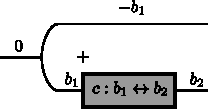
\includegraphics{diagrams/function.pdf}
\end{center}

Let us use the shorthand {{b1 -o b2 = -b1 + b2}}

\paragraph*{Function application}

\begin{center}
  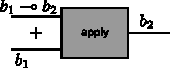
\includegraphics{diagrams/apply1.pdf}
\end{center}

\begin{center}
  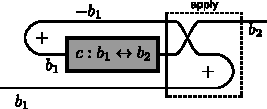
\includegraphics{diagrams/apply2.pdf}
\end{center}

\paragraph*{Function composition}

\begin{center}
  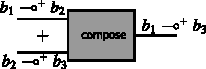
\includegraphics{diagrams/compose1.pdf}
\end{center}

\begin{center}
  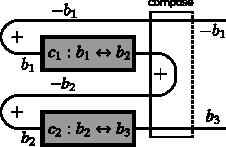
\includegraphics{diagrams/compose.pdf}
\end{center}

This is also equivalent to sequencing both the computation blocks. 

\begin{center}
  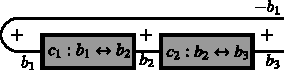
\includegraphics{diagrams/compose2.pdf}
\end{center}


\paragraph*{Delimited continuation}

\begin{center}
  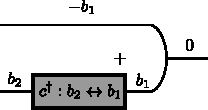
\includegraphics{diagrams/delimc.pdf}
\end{center}

\paragraph*{Trace }

%subcode{proof} include main
%@ c : b2 + b1 <-> b2 + b3
%@@ trace c : b1 <-> b3

\begin{center}
  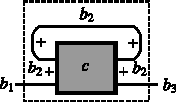
\includegraphics{diagrams/trace.pdf}
\end{center}

\paragraph*{Principium Contradictiones}

{{b <-> -(-b)}}

\begin{center}
  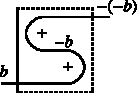
\includegraphics{diagrams/double_neg.pdf}
\end{center}

MUST TALK ABOUT AND CITE ABRAMSKY AND COECKE'S TR ABOUT QUANTUM
COMPUTING.


%%%%%%%%%%%%%%%%%%%%%%
\subsection{Constructions Specific to Negation}
\label{sec:neg-constructions}

\paragraph*{Negation distributes over {{+}}. }

{{-(b1 + b2) <-> (b1) + (-b2)}}

\begin{center}
  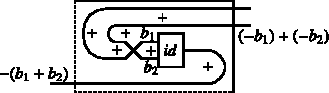
\includegraphics{diagrams/dist_neg_plus.pdf}
\end{center}

\paragraph*{ {{eps_{fst} }} }

{{(-b1)*b2 + b1*b2 <-> 0}}

\begin{center}
  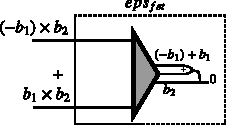
\includegraphics{diagrams/eps_fst.pdf}
\end{center}

\paragraph*{Lifting negation out of {{*}}. }

{{(-b1) * b2 <-> -(b1 * b2) <-> b1 * (-b2)}}

\begin{center}
  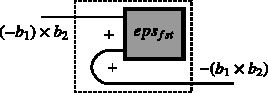
\includegraphics{diagrams/mult_neg.pdf}
\end{center}

The following isomorphism can be constructed similarly 

{{b1 * b2 <-> (-b1)*(-b2)}}


\paragraph*{Lifting a operation of positive types to negated types}

Given {{c : b1 <-> b2}}

\begin{center}
  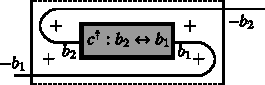
\includegraphics{diagrams/neg_lift.pdf}
\end{center}


%%%%%%%%%%%%%%%%%%%%%%
\subsection{Constructions Specific to Multiplication}


%%%%%%%%%%%%%%%%%%%%%%
\subsection{To think about}

\begin{itemize}

\item If we built an effect over {{langRevEE}}, say {{create}} and
  {{erase}}, are effects structured by an arrow or a monad now?

\item Which operations can be lifted to work on negative types?

\item Can the operational semantics for {{langRevEE}} be an
  interpreter that is implemented in {{langRevT}} (similar to how the
  the tree traversal interpreter was implemented). This would imply
  the existence of a more powerful construction than Int, wherein the
  products would also be preserved. This is possibly worth a paper in
  itself.

\item These functions aren't really values. There is no value one can
  produce that denotes a function. These functions are the ability to
  transform a value - the possibility of transforming a value.  In the
  product encoding of environments, there is no value one can assign
  to a variable such that it denotes a function.


Actually this is possible. Consider two functions {{f : b1 <-> b2}}
and {{g : b1 <-> b2}}. A value of type {{bool}} is sufficient to
discriminate them. Hence the {{boo}} is the first class representation
of the functions and can be thought of as the address of the function. 

\begin{center}
  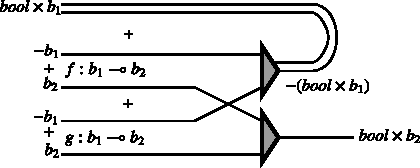
\includegraphics{diagrams/dispatch.pdf}
\end{center}


\item It is not fair to say that negative types flow backwards. The
  following circuits are valid in {{langRevEE}}. It is however proper
  to say that for any type {{b}} that flows in a direction, the type
  {{-b}} flows in the reverse direction. 

\begin{center}
  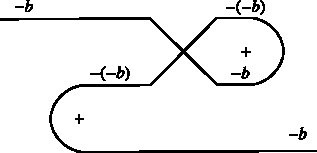
\includegraphics{diagrams/neg_circuit1.pdf}
\end{center}

\begin{center}
  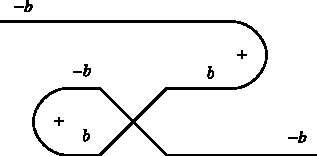
\includegraphics{diagrams/neg_circuit2.pdf}
\end{center}

\end{itemize}

For a traced monoidal category {{C}} the Int construction produces a
Compact Closed Category called Int {{C}} \cite{joyal1996traced}.
Further we know that the target of the Int construction is isomorphic
to the target of \G construction of Abramsky \cite{Abramsky96:0} from
Haghverdi. However, note that the {{langRevEE}} is not the same as the
image of the Int construction on {{langRevT}}, since the the later
lacks a multiplicative tensor that distributes over the additive tensor
in Int {{langRevT}}.

%%%%%%%%%%%%%%%%%%%%%%%%%%%%%%%%%%%%%%%%%%%%%%%%%%%%%%%%%%%%%%%%%%%%%%%%%%%%%%%%
\section{Advanced Programming Examples}
\label{sec:prog}

%%%%%%%%%%%%%%%%%%%
\subsection{SAT solver}
\label{sec:sat-solver}

The construction presented here is a novel SAT-solver that relies on
{{trace*}} for its solution. It varies from previous classical SAT
solvers in that there is not explicit search operation on the boolean
space. It also varies from previous quantum SAT solvers in that it
does uses a {{trace}} operation to compute a fixpoint which is the
solution following which an isomorphic clone operation allows us to
examine the result.

The construction here is not limited to boolean satisfiability, but
generalizes to any constraint satisfaction problem whose search space
can be represented by a recursive type and for which an isomorphic
clone operation can be constructed. That said, we will focus on the
limited case of boolean satisfiability here. 

Consider the circuit below that has no observable output -- i.e. for
all inputs it is annihilating. This happens because it constructs a
boolean and its dual, negates one of them and attempts to collapse
them.
\begin{center}
\scalebox{1.2}{
  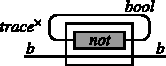
\includegraphics{diagrams/not_trace.pdf}
}
\end{center}  

We leverage the basic idea of the above circuit, to collapse all
values that are not solutions to the specified isomorphic constraint
{{f}}. The contraint {{f}} checks the inputs to see if they match a
constraint -- in the case of the SAT solver, {{f}} would be the
circuit expressing the boolean expression to be satisfied.  While the
output of {{f}} may contain many components, its must contain a
boolean indicating if the input satisfy {{f}}. The operation {{f}}
acts on some inputs and its adjoint, {{f^{dagger} }}, reconstructs the
inputs from the outputs.  The `trick' is the following: the special
output wire is used to `control' the negation of a boolean `control
wire'.  If the inputs do not satisfy {{f}}, the control wire is
negated.

\begin{center}
\scalebox{1.5}{
  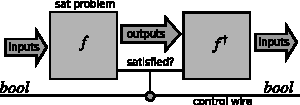
\includegraphics{diagrams/sat1.pdf}
}
\end{center}  

If this construction is traced using {{trace*}}, all the values that
do not satisfy {{f}} get annihilated because the control wire acts
like the closed-loop `not' in the previous construction. 

The final detail we have to be concerned with is the handling of the
heap and garbage of {{f}}. Any boolean expression {{bool^n -> bool}}
can be compiled into the isomorphism {{f:bool^h*bool^n<->bool^g*bool}}
where the extra bits {{bool^h}} and {{bool^g}} are the heap and
garbage. Constructing such an isomorphism has been detailed before
\cite{Toffoli:1980,infeffects}.  However the computation of {{f}} is
meaningful {{iff}} the heap {{bool^h}} is initialized appropriately. We
can ensure that the heap has the appropriate initial value by checking
the heap and negating a second control wire, if the values do not
match.

\begin{center}
\scalebox{1.5}{
  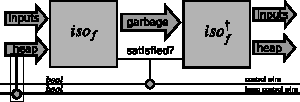
\includegraphics{diagrams/sat2.pdf}
}
\end{center}  



%%%%%%%%%%%%%%%%%%%
\subsection{GoI machine}

We can now encode the GoI machine of
Mackie~\cite{Mackie2011,DBLP:conf/popl/Mackie95}. \amr{The machine uses bang
  which allows arbitrary duplication. Can we really do that???}

%%%%%%%%%%%%%%%%%%%%%%%%%%%%%%%%%%%%%%%%%%%%%%%%%%%%%%%%%%%%%%%%%%%%%%%%%%%%%%%%
\section{Related Work} 
\label{sec:related}

The idea of ``negative types'' has appeared many times in the literature and
has often been related to some form of continuations. Fractional types are
less common but have also appeared in relation to parsing natural
languages. Although each of these previous occurrences of negative and
fractional types is somewhat related to our work, our results are
subtantially different. To clarify this point, we start by reviewing the
salient point of the major pieces of related work and conclude this section
with a summary contrasting our approach to previous work.

\paragraph*{Declarative Continuations.} 
In his Masters thesis~\cite{Filinski:1989:DCI:648332.755574}, Filinski
proposes that continuations are a \emph{declarative} concept. He,
furthermore, introduces a symmetric extension of the $\lambda$-calculus in
which call-by-value is dual to call-by-name and values are dual to
continuations. In more detail, the symmetric calculus contains a ``value''
fragment and a ``continuation'' fragment which are mirror images. Pairs and
sums are treated as duals in the sense that the ``value'' fragment includes
pairs whose mirror image in the ``continuation'' fragment are sums. In
contrast, our language includes pairs and sums in the value fragment and two
symmetries: one that maps the pairs to fractions and another that maps the
sums to subtractions.

\paragraph*{The Duality of Computation.}
The duality between call-by-name and call-by-value was further investigated
by Selinger using control
categories~\cite{Selinger:2001:CCD:966910.966911}. Curien and
Herbelin~\cite{Curien:2000} also introduce a calculus that exhibits
symmetries between values and continuations and between call-by-value and
call-by-name. The calculus includes the type $A-B$ which is the dual of
implication, i.e., a value of type $A-B$ is a context expecting a function of
type $A \rightarrow B$. Alternatively a value of type $A-B$ is also explained
as a \emph{pair} consisting of a value of type $A$ and a continuation of type
$B$. This is to be contrasted with our interpretation of a value of that type
as \emph{either} a value of $A$ or a demand for a value of type $B$. This
calculus was further analyzed and extended by
Wadler~\cite{Wadler:2003,DBLP:conf/rta/Wadler05}. The extension gives no
interpretation to the subtraction connective and like the original symmetric
calculus of Filinksi, introduces a duality that relates sums to products and
vice-versa.

\paragraph*{Subtractive Logic.} 
Rauszer~\cite{springerlink:10.1007/BF02120864,rauszer,rauszer2} introduced a
logic which contains a dual to implication. Her work has been distilled in
the form of \emph{subtractive logic}~\cite{Crolard01} which has recently been
related to coroutines~\cite{Crolard01082004} and delimited
continuations~\cite{Ariola:2009:TFD:1743339.1743381}.  In more detail,
Crolard explains the type $A-B$ as the type of \emph{coroutines} with a local
environment of type $A$ and a continuation of type $B$. The description is
complicated by what is essentially the desire to enforce linearity
constraints so that coroutines cannot access the local environment of other
coroutines. 

\paragraph*{Negation in Classical Linear Logic} 
Filinski~\cite{Filinski92} uses the negative types of linear logic to model
continuations. Reddy~\cite{Reddy91} generalizes this idea by interpreting the
negative types of linear logic as \emph{acceptors}, which are like
continuations in the sense that they take an input and return no
output. Acceptors however are also similar in flavor to logical variables:
they can created and instantiated later once their context of use is
determined. Although a formal connection is lacking, it is clear that, at an
intuitive level, acceptors are entities that combine elements of our negative
and fractional types.

\paragraph*{The Lambek-Grishin Calculus.} The ``parsing-as-deduction'' style
of linguistic analysis uses the Lambek-Grishin calculus with the following
types: product, left division, right division, sum, right difference, and
left difference~\cite{Bernardi:2010:CSL:1749618.1749689}. The division and
difference types are similar to our types but because the calculus lacks
commutativity and associativity and only has limited notions of
distributivity, each connective needs a left and right version. The
Lambek-Grishin exhibits two notions of symmetry but they are unrelated to our
notions. In particular, the first notion of symmetry expresses commutativity
and the second relates products to sums and divisions to subtractions. In
contrast, our two symmetries relate sums to subtractions and products to
divisions.

\paragraph*{Our Approach.} The salient aspects of our approach are the following:
\begin{itemize}
\item Negative and fractional types have an elementary and familiar
  interpretation borrowed from the algebra of rational numbers. One can write
  any algebraic identity that is valid for the rational numbers and interpret
  it as an isomorphism with a clear computational interpretation: negative
  values flow backwards and fractional values represent fragments of
  aggregate data structures. None of the systems above has such a natural
  interpretation of negative and fractional types. 
\item Because we are \emph{not} in the context of the full
  $\lambda$-calculus, which allows arbitrary duplication and erasure of
  information, values of negative and fractional types are first-class values
  that can flow anywhere. The information-preserving computational
  infrastructure guarantees that, in a complete program, every negative
  demand will be satisfied exactly once, and every constraint imposed by a
  fractional value will also be satisfied exactly once. This property is
  shared with systems that are based on linear logic; other systems must
  impose ad hoc constraints to ensure negative values are used exactly
  once. 
\item In contrast to all the work that takes continuations as primitive
  entities of negative types, we view continuations as a derived notion that
  combines a demand for a value with constraints on how this value will be
  used to proceed with the evaluation (to the closest delimiter or to the end
  of the program). In other words, we view a continuation as a non-elementary
  notion that combines the negative types to demand a value and the
  fractional types to explain how this value will be used to continue the
  evaluation. As a consequence, the previously observed duality between
  values and continuations can be teased into two dualities: a duality
  between values flowing in one direction or the other and a duality between
  aggregate values composing and decomposing into smaller values. Arguably
  each of the dualities is more natural than a duality that maps regular
  values to a conflated notion of negative and fractional types, and hence
  requires notions like ``additive pairs'' and ``multiplicative sums.''
\end{itemize}

%%%%%%%%%%%%%%%%%%%%%%%%%%%%%%%%%%%%%%%%%%%%%%%%%%%%%%%%%%%%%%%%%%%%%%%%%%%%%%%%
\section{Conclusion}
\label{sec:conc}

The field of algebraic numbers consist of the rationals extended with
solutions to polynomials. In a limited sense {{langRevEE}} with
recursive types already include polynomials such as the definition of
binary tree {{@@x.(1+x*x)}} implies the equality {{t = 1 + t*t}} and
hence {{t^2-t+1=0}}. While this equation does indeed have an
irrational imaginary root, as we will see -- {{langRevEE}} does not
have the means of expressing meaningful computation that uses the
root.

Here is one way to view computations involving irrationals that might
shed some insight into how we should view recursive data types
also. For finite datatypes say of size {{n}} we can say that an
element specifies a choice of {{1/n}} and hence contains as much
information. For finite things, each value is computationally equal to
any other value. Any permutation is possible among the values. Hence
there is no metric possible on the values.  Recursive data types, such
as binary trees, have an infinite number of elements and hence the
argument that says that value specifies {{1/n}} units of information
is not longer valid. Instead to talk meaningfully about information
content, we should talk about a probability distribution on the values
of the type. However what shall we base this distribution on? Is there
a natural order beyond the unfolding order of the values of a type? 

In this context, let us go back to the thought that recursive such as
{{nat=nat+1}} have no meaningful solutions, whereas trees do. But the
interesting solution of trees is precisely that they involve
irrational numbers. Our usual notation for irrationals such as
{{sqrt(2) }} can actually be viewed as a thunk representing the
infinite computation {{1.4142..}}. Irrationals in this sense have a
very different information theoretic interpretation from full real
numbers. With Chaitin's Omega numbers he postulates the existence of
real numbers that have an infinite amount of information -- ones for
example are the solution to the question about the halting properties
of every Turning machine. 

Real numbers in that sense really are a series of bits of unknown
information theoretic interpretation -- a sort of {{top}}. Numbers
such as {{sqrt(2) }} are very different in the sense that even though
they contain an infinite sequence of bits, there is a finite program
that generates those bits and its only the cost of computing bits that
is infinite.  The consistency of arithmetic isn't affected by
extending the rational field by adding any specific computable
irrational. So it might be possible to design a model of computing
where we can indeed deal with them. Such a model will have to explicit
thunks for the delayed computation represented by trees and never
equate and cancel two infinite computations unless the represent
exactly the same infinite computation.

TODO.

Square root and imaginary types have also appeared in the literature: we
relegate the connections to Sec.~\ref{sec:related} and proceed with a simple
explanation. We have so far extended the set of types to be the rational
numbers. Now we will push this and extend the set of types to algebraic
numbers. In other words, we will allow datatypes defined by arbitrary
polynomials and allow the roots of such polynomials to be types. 

Consider first an example in which we want to compute with the sides of a
rectangle whose area is 91 and whose length is longer than its width by 6
units. One can solve the quadratic equation to determine that the sides are 7
and 13 and proceed. This however prematurely forces us to globally solve the
constraint. Instead we can let the two sides of the rectangle be $x$ and
$x+6$ and use the following equation to capture the desired constraint:
\[
x^2 + 6x - 91 = 0
\]
The equation introduces an isomorphism between the type $x^2 + 6x - 91$ and
the type $0$. We can now proceed to compute with the unknown $x$, being
assured that in a closed program, our computation will eventually be
consistent with the solution of the algebraic equation. 

Previously the most famous example of a similar nature is the puzzling
isomorphism that one can establish between seven binary trees and one.
A binary tree is defined by the datatype
\[
x = 1 + x * x 
\]
which can be rearranged to the polynomial equation $x^2 - x + 1 = 0$. By
algebraic manipulation we can reason as follows:
\[\begin{array}{rclclclcl}
x^3 &=& x^2 x &=& (x-1) x &=& x^2 - x &=& -1 \\
x^6 &=& 1 \\
x^7 &=& x^6 x &=& x
\end{array}\]
Fiore poses the question of why such algebraic manipulation would make sense
type theoretically but states that even though some of the intermediate steps
make no sense, the final equivalence is valid and can be used to actually
construct an isomorphism between $x^7$ the type of seven binary trees 
and $x$ the type of binary trees.

Discussion of possible polynomials:
\begin{itemize}
\item $b=1+1$. Boring.
\item $b=b+1$. That introduces the natural numbers. No solution for this
  polynomial over the algebraic numbers. We must extend the numbers with
  $\omega$ to get a solution. We reject this in this paper and prefer to
  stick to algebraic numbers. The advantage is that all the isomorphisms are
  valid numerically. With the above type we could subtract $b$ from both
  sides to show that $0=1$ which is nonsense. We can however have infinite
  types as long as they have algebraic solutions.
\item $b^2=2$ or $b = \pm \sqrt{2}$. We have introduced the square root of a
  boolean! If we had superpositions, we could then write a function that
  performs the square root of negation in the sense that applying it twice
  would be equivalent to boolean negation.
\end{itemize}

To summarize negative, fractional, square root, and imaginary types all make
sense. What they help you accomplish as a programmer is to disassociate
global invariants into local ones that can be satisfied independently by
subcomputations with no synchronization or communication. A computation
producing something of type $a/b$ does not need to concern itself with who is
going to supply the missing $b$: it just does its part. Conversely faced with
a complicated task, a computation might decide to break it into pieces and
demand these pieces using negative types. 

It is no surprise that these types are closely related to quantum mechanics
and that they give us the feel that this is how nature computes. This is
speculation however.

In any case, in a framework where information can be copied and deleted, none
of this makes much sense. It is critical that these constraints and demands
can neither be duplicated nor erased.  This gives us the maximum
``parallelism'' possible.

In our previous work we introduce recursive types and trace operators. This
is dangerous here because infinite loops allow us to prolong paying the debt
for as long as we want. The algebraic
$\lambda$-calculus~\cite{Vaux:2009:ALC:1630585.1630590} shows that extreme
care is needed when combining negative and fractional types with the full
$\lambda$-calculus (including recursion).

Say we have not considered recursion in this paper.

The simplest way to connect the In a conventional computational model, one
might realize this situation by simply writing the identity function: the
buyer hands the money to the seller to finish the transaction. The above
sequence of isomorphisms implements this identity function in a much more
interesting way, however.  of the above series of

On the producer side, the debt is paid for by the money computation with the
identity function. the producer and consumer must somehow share an explicit
dependency that allows the value. However in our model, the presence of
negative types allows the produced value to satisfy the demand without the
producer or consumer even knowing about each other. As is explained in detail
in

Furthermore, we illustrate their true appeal and expressiveness is brought
forth by viewing them in the context of an information-preserving
computational model.

In addition, we show how these types enrich our computational model, they
obey the same laws as the rational numbers. In other words, every algebraic
identity that holds for the rational numbers corresponds to a type
isomorphism in our model.

Specifically, isomorphisms enrich our computational model with have an
interesting computational interpretation

In particular, linear logic~\cite{Girard87tcs}, among other contributions,
exposed an additive/multiplicative distinction in logical connectives and
rules. In particular, linear logic includes additive disjunctions $\oplus$
and conjunctions $\with$ as well as multiplicative disjunctions $\parr$ and
conjuctions $\otimes$. Duality is also prominent in linear logic: it relates
the additive connectives to each other (the dual of $\oplus$ is $\with$ and
vice-versa) and the multiplicative connectives to each other (the dual of
$\otimes$ is $\parr$ and vice-versa).

We furthermore demonstrate that, in our model,
programming with these negative and fractional types, is a new ``revolution''
breaking dependencies...

Since Filinski, we've had the
idea that values and continuations are like mirror images. In a conventional
language, the negative (continuation) side is implicit and we introduce
information effects on the positive. Trying to recover the duality from this
distorted positive side has always been messy. Now it looks clean because we
have kept the positive side pure.

Continuations made their introduction to the world of programming language
semantics as a mathematical device to model first-class labels and
jumps~\cite{springerlink:10.1023/A:1010026413531}. In a remarkable
development, Filinski~\cite{Filinski:1989:DCI:648332.755574} observed that
--- with the right perspective --- this highly imperative concept was
actually the symmetric dual of values. The heart of the observation is that
values represent entities that flow from producers to consumers while
continuations represent \emph{demands} for such entities, that flow from
consumers to producers. In more detail, Filinski describes continuations as
representing ``the \emph{lack} or \emph{absence} of a value, just as having a
negative amount of money represents a debt.'' He then proceeds to construct a
language where values and continuations are treated truly symmetrically. To
that end, he abandons the $\lambda$-calculus amalgamation of functions and
values and distinguishes between three different syntactic classes:
functions, values, and continuations, with the property that any function can
be used either as a value transformer or as a continuation transformer.

This highly intuitive and appealing idea was further explored and refined by
many authors~\cite{Griffin:1989:FNC:96709.96714, Curien:2000,
  Wadler:2003, DBLP:conf/rta/Wadler05}. Yet, despite its appeal, the duality
between values and continuations 

Computationally, symmetry exhibits itself as a duality between two concepts.

Symmetry is pervasive in both natural and man-made environments. 

In 1989, Filinski~\cite{Filinski:1989:DCI:648332.755574} observed that values
and continuations are dual notions. This observation was followed by numerous

We introduced this thesis that computation should be based on isomorphisms
that preserve information~\cite{infeffects}. Since Filinski, we've had the
idea that values and continuations are like mirror images. In a conventional
language, the negative (continuation) side is implicit and we introduce
information effects on the positive. Trying to recover the duality from this
distorted positive side has always been messy. Now it looks clean because we
have kept the positive side pure.

In a technical sense, this paper extends the language of isomorphisms
{{langRev}}, with duality. Unlike Linear logic \cite{Girard87tcs} and
other systems which have one notion of duality over additive and
multiplicative components, {{langRevEE}} has two notions of duality
-- an additive duality over the monoid {{(0, +)}} and a multiplicative
duality over the monoid {{(1, *)}}. Each axis of duality also give us
a function space and hence {{langRevEE}} has an additive function
space corresponding to a notion of control or backtracking and a
multiplicative function space corresponding to a notion of unification
or constraint satisfaction.

The world of computation we are describing has:
\begin{itemize}
\item suppliers, 
\item consumers, and
\item bi-directional transformations
\end{itemize}
This is the same world described by the papers on the duality of computation
but that work only scratched the surface! We have the following features:
\begin{itemize}
\item we can start from the supplier and push the values towards the
  consumer (call-by-value in the duality of computation papers)
\item we can start from the consumer and pull the values from the suppliers
  (call-by-name in the duality of computation papers)
\item we can combine the pushing and pulling and values using eta/epsilon for
  sum types; these allow us to at any point in the middle of the computation
  create out of nothing a value to send to the consumers and a demand to send
  to the suppliers.
\item we can break a big data structure into fragments described by
  fractional types; the suppliers and consumers can produce and consume the
  pieces completely independently of each other. Eventually the pieces will
  fit together at the consumer to produce the desired output.
\item we can break a bi-directional transformation into pieces using square
  roots
\item we can take into account that values have phase (complex numbers),
  i.e., it is not that they flow towards the consumer or just towards the
  suppliers; they can be flowing in direction that ``30 degrees'' towards the
  consumer for example.
\end{itemize}
So it is all about breaking dependencies in some sense to allow for maximum
autonomy (parallelism) of subcomputations. It is probably the case that to
make full use of square root types and imaginary types, we have to move to a
vector space. If that's the case, we should probably leave this stuff out and
focus on negative and fractional types and only have a short discussion of
the polynomials restricted to seven trees in one and similar issues.

The conventional idea is to divide the world into a ``real'' one and a
``virtual'' one. In the ``real'' world, we can define datatypes like
\verb|t=t^2+1| but we don't have additive inverses so it makes no sense to
talk of negative types and we can't rearrange the terms in the datatype
definition. However the observation is that we can map these datatypes to a
virtual world that has more structure (a ring that provides additive inverses
or a field that also provides multiplicative inverses) and then perform
computations in the ring/field. If we perform computations in the ring, then
some of these will use additive inverses in ways that cannot be mapped back
to the ``real'' world. Much of current research attempts to characterize
which computations done in the ring are valid isomorphisms between datatypes
in the ``real'' world. This is nice but is not what I am after. In fact I am
not interested in the ring or the semiring at all. I am interested in the
field and I want this field to be \textbf{the real world.} This is partly
motivated by the fact that Quantum Mechanics seems to demand an underlying
field and more generally that the field provides the maximum generality in
slicing and dicing computations. So assuming I live in a field and that the
negative, fractional, square root, and imaginary types are all ``real,'' how
do I compute in this field? Clearly there will be constraints on
``measurement'' in the sense that a full program cannot produce any of the
crazy types but that's done outside the formalism in some sense just as in
Quantum Computing. The main question I am after is how to compute in this
field with first-class negative, fractional, etc. types. As I mentioned in my
previous email, we can produce programs that have types \verb|t^3 <-> -1| and
they ``run'' (but only to give infinite loops). 

So when a programmer writes the datatype declaration \verb|t = t^2+1|,
if we allow negative etc. then this is effectively writing
\verb|t = cubicroot{-1}|. If we are in the field then computations
that manipulate these trees can be sliced and diced even at interfaces
that expose the cubic root and the imaginary types.

Future work: develop a type system for a ``normal language'' that has
negative, fractional, etc. types as first-class types. More long term,
instead of adding one polynomial at a time, we can go to an algebraically
closed field. The complex numbers is an obvious choice but I would rather go
to something computable like the field of algebraic numbers. Is the adele
ring or the p-adics relevant here?


We show a deep symmetry between functions and delimited continuations, values
and continuations that arises in {{langRev}} in a manner that is reminiscent
of Filinksi's Symmetric \lcal ~\cite{Filinski:1989:DCI:648332.755574}. The
symmetry arises by extending {{langRev}} with a notion of additive duality
over the monoid {{(+, 0)}} by including {{eta+}} and {{eps+}} operators of
Compact Closed Categories. The resulting dual types, which we denote {{-b}},
have a time traveling ``backward information flow'' interpretation and allow
for the encoding of higher-order function and iteration via the construction
of trace operators, thereby making the extended language {{langRevEE}} a
Turing-complete reversible programming language with higher-order functions
and first-class delimited continuations.

We introduced this thesis that computation should be based on isomorphisms
that preserve information~\cite{infeffects}. Since Filinski, we've had the
idea that values and continuations are like mirror images. In a conventional
language, the negative (continuation) side is implicit and we introduce
information effects on the positive. Trying to recover the duality from this
distorted positive side has always been messy. Now it looks clean because we
have kept the positive side pure.

The way to think about something of type $A$ is that it is a value we have
produced. The way to think about something of type $-A$ is that is a value we
have already consumed. 

Other interpretations of the types of think about. The first one is
arithmetic obviously. Another one is languages consisting of sets of
string. The type 0 is the empty set, the type 1 is the set containing the
empty word, the $+$ constructor corresponds to union, and the $*$ constructor
corresponds to concatenation. The constructor $-$ would not correspond to set
difference however. It would correspond to marking the elements in the set as
``consumed'' so that if we take the union and a ``consumed'' element appears
in the other set, the two cancel. This makes it clear that concatenating a
produced $a$ and a consumed $b$ is not the same as concatenating a consumed
$a$ and a produced $b$. They really need to be kept separate. Incidentally,
division would be defined as follows:
\[
L_1 / L_2 = \{ x ~|~ xy \in L_1 \mbox{~for~some~} y \in L_2 \}
\]

Filinski proposes that continuations are a \emph{declarative} concept. He,
furthermore, introduces a symmetric extension of the $\lambda$-calculus in
which values and continuations are treated as opposites. This is essentially
what we are proposing with one fundamental difference: our underlying
language is not the $\lambda$-calculus but a language of pure isomorphisms in
which information is preserved. This shift of perspective enables us to
distill and generalize the duality of values and continuations: in
particular, in the conventional $\lambda$-calculus setting values and
continuations can be erased and duplicated which makes it difficult to
maintain the correspondence between a value and its negative counterpart.

The idea of using negative types to model information flowing backwards,
demand for values, continuations, etc. goes back to at Filinski's thesis. We
recall these connections below but we first note that all these systems are
complicated because in all these systems information can be ignored,
destroyed, or duplicated. Clearly the possibility of erasure of information
would mean that our credit card transaction is incorrect. In our work,
information is maintained and hence we have a guarantee that, in a closed
program, the debt must be accounted and paid for.

Much of previous work builds on the idea that there is one duality in
computation between values and continuations which manifests itself as a
duality between the call-by-value and call-by-name parameter-passing
mechanisms. The former mechanism focuses on evaluating expressions to values
even if these values are not demanded by the context; the latter focuses on
evaluating expressions to continuations even if these continuations might be
aborted. The idea that a continuation is dual to a value is intuitive but
then one would expect that the sum of two values naturally corresponds to the
sum of two continuations and that the product of two values naturally
corresponds to the product of two continuations.

check and say that our work teases the continuations into a negative part
(which simply demands a value) and a fractional part (which imposes
constraints on how this value will be used). So something like $-1/c$ is
needed to express a conventional continuation. Having two dualities makes the
whole calculus natural and symmetric.

Consider a continuation that takes $x$ and $y$ and swaps them. It can't be
expressed using two conventional continuations because the demand and the way
it is used are entangled together.

In accounts that are linear, the value and continuation that comprise the
subtractive type need to be constrained to ``stay together.'' This can be
achieved by various restrictions. In this work we have no such constraints,
the negative value can flow anywhere. The entire system guarantees that any
closed program would have to account for it. We don't have to introduce
special constraints to achieve that. Zeilberger in the paper on polarity and
the logic of delimited continuations uses polarized logic: he shows that if
positive and negative values are completely symmetric except that answer
types are positive, then the framework accommodates delimited
continuations. But he interprets negative values are control operators, or as
values defined by the shape of their continuations. We simply interpret
values of negative type as values flowing in the ``other'' direction.

This is essentially what we are proposing with one fundamental difference:
our underlying language is not the $\lambda$-calculus but a language of pure
isomorphisms in which information is preserved. This shift of perspective
enables us to distill and generalize the duality of values and continuations:
in particular, in the conventional $\lambda$-calculus setting values and
continuations can be erased and duplicated which makes it difficult to
maintain the correspondence between a value and its negative counterpart. In
contrast, in our setting, one can start from the empty type $0$, introduce a
positive value and its negative counterpart, and let each of these flow in
arbitrary ways. The entire framework guarantees that neither the value nor
its negative counterpart will be deleted or duplicated and hence that, in any
closed program, the ``debt'' corresponding to the negative value is paid off
exactly once. The forward and backward executions in our framework correspond
to call-by-value and call-by-name. This duality was observed by Filinski and
others following him but it is particularly clean in our framework.

%% Jacques

\acks This project was partially funded by Indiana University's Office
of the Vice President for Research and the Office of the Vice Provost
for Research through its Faculty Research Support Program.  We also
acknowledge support from Indiana University's Institute for Advanced
Study.

%%%%%%%%%%%%%%%%%%%%%%%%%%%%%%%%%%%%%%%%%%%%%%%%%%%%%%%%%%%%%%%%%%%%%%%%
\begin{small}
\bibliographystyle{abbrvnat}
\bibliography{cites}
\end{small}


\end{document}

%%%%%%%%%%%%%%%%%%%%%%%%%%%%%%%%%%%%%%%%%%%%%%%%%%%%%%%%%%%%%%%%%%%%%%%%
